\ifdefined\ishandout
\documentclass[handout]{beamer}
\else
\documentclass{beamer}
\fi

\usepackage[frenchb]{babel}
\usepackage[T1]{fontenc}
\usepackage[latin1]{inputenc}
\usepackage{hyperref}
\usepackage{multirow}
\usepackage{listings}
\usepackage{fancyvrb}
\usepackage{tikz}
\usepackage{framed}
\usepackage{algorithm}
\usepackage{algorithmic}
\usepackage{xcolor}
\usepackage{color, colortbl}
\usepackage{handoutWithNotes}
\usetikzlibrary{shapes.geometric}
\usetikzlibrary{shapes.arrows, chains}
\usetikzlibrary{arrows,calc}
\usepackage{array}
\usetheme{Boadilla}

\ifdefined\ishandout
\pgfpagesuselayout{3 on 1 with notes}[a4paper,border shrink=5mm]
\usecolortheme{dove}
\else
\usecolortheme{dolphin}
\fi


\lstnewenvironment{codeC}
{ \lstset{language=C,
    otherkeywords={printf,scanf}}
}
{}

\ifdefined\ishandout
\definecolor{mygreen}{rgb}{0,0,0}
\definecolor{mymauve}{rgb}{0,0,0}
\definecolor{myblue}{rgb}{0,0,0}
\else
\definecolor{mygreen}{rgb}{0,0.6,0}
\definecolor{mymauve}{rgb}{0.58,0,0.82}
\definecolor{myblue}{rgb}{0,0,1}

\fi

\definecolor{mygray}{rgb}{0.5,0.5,0.5}


\lstset{language=C,
% breakatwhitespace=false,         % sets if automatic breaks should only happen at whitespace
%  breaklines=true,                 % sets automatic line breaking
%  captionpos=b,                
commentstyle=\itshape\color{mymauve},
keywordstyle=\bfseries\color{myblue},
%numbers=left,                    % where to put the line-numbers; possible values are (none, left, right)
%  numbersep=8pt,                   % how far the line-numbers are from the code
%  numberstyle=\tiny\color{mygray}, % the style that is used for the line-numbers
  rulecolor=\color{black},         % if not set, the frame-color may be changed on line-breaks within not-black text (e.g. comments (green here))
%  showspaces=false,                % show spaces everywhere adding particular underscores; it overrides 'showstringspaces'
  showstringspaces=false,          % underline spaces within strings only
%  showtabs=false,                  % show tabs within strings adding particular underscores
%  stepnumber=2,                    % the step between two line-numbers. If it's 1, each line will be numbered
  stringstyle=\color{mygreen},     % string literal style
%  tabsize=2 
}

\newcommand{\red}{\textcolor{red}}
%\newcommand \emph
%Default size : 12.8 cm * 9.6 cm

\ifdefined\ishandout
\newenvironment<>{codeblock}[1]{%begin
  \setbeamercolor{block title}{fg=black,bg=lightgray!80}%
  \begin{block}{#1}}
  % \begin{codeC}}
  %  {\end{codeC}
{  
\end{block}}

\newenvironment<>{termblock}[1]{
    \setbeamercolor{block title}{fg=black,bg=lightgray!90}%
    \begin{block}{#1}
}
%     \begin{Verbatim}}
{%\end{Verbatim}
\end{block}
}

\definecolor{bluegreen}{RGB}{0,0,0}
%\definecolor{bluegreen}{rgb}{0,0.6,0.8}
\else

\newenvironment<>{codeblock}[1]{%begin
  \setbeamercolor{block title}{fg=darkgray,bg=yellow}%
  \begin{block}{#1}}
  % \begin{codeC}}
  %  {\end{codeC}
{  
\end{block}}

\newenvironment<>{termblock}[1]{
    \setbeamercolor{block title}{fg=white,bg=lightgray}%
    \begin{block}{#1}}
%     \begin{Verbatim}}
{%\end{Verbatim}
\end{block}
}

\definecolor{bluegreen}{RGB}{0,149,182}
%\definecolor{bluegreen}{rgb}{0,0.6,0.8}
\fi

%\newcommand{\output}[1]{
\setbeamertemplate{navigation symbols}{}
\newcommand{\bvrb}{\Verb[commandchars=���,formatcom=\color{bluegreen}]}



%%% Param�tres du cours (� r�gler)
%Num�ro du cours
\newcommand{\nb}{3}

\title[Cours n�\nb]{Cours n�\nb - Compilation/Tableaux/IO}
\author[]{julien.brajard@upmc.fr}
\institute[Polytech' UPMC]{Polytech' UPMC}
\date{12 Octobre 2015}
\begin{document}
%%%%%%%%%%%%%%%%%%%%% SLIDES DE TITRE
\begin{frame}
\titlepage
\centering{
\url{http://australe.upmc.fr} (onglet EPU-C5-IGE Info Gen)}
\end{frame}
%%%%%%%%%%%%%%%%%%%%%
\begin{frame}
\frametitle{Plan du cours n�\nb}
\tableofcontents[hideallsubsections]
\end{frame}

%%%%



%%%%%% SECTION 12
% !TEX encoding = IsoLatin9

%%%%%%%%%%%%%%%%%%%%% SECTION 1
\section{La compilation}
\begin{frame}
  \begin{columns}
    \column{4.8cm}
    \tableofcontents[currentsection,hideothersubsections]
    \column{7cm}
    
  \end{columns}
  
\end{frame}

%%%%%%%%%%%%%%%%%%%%%%%%%%%%%%%%%%%%%%%%%%%
%                  FRAME 1                %
%%%%%%%%%%%%%%%%%%%%%%%%%%%%%%%%%%%%%%%%%%%

\begin{frame}[t,fragile]
\frametitle{Les 4 �tapes de la compilation}

%%%%%%%%%%%%%% ALL SLIDES %%%%%%%%%%%%%%%%%%
\vspace{-0.7cm}
\begin{figure}[t]
\centering
\begin{tikzpicture} [
  block/.style    = { rectangle, draw=blue, thick, 
                      fill=blue!20, text width=1.8cm, text centered,
                      rounded corners, minimum height=2em },
 ablock/.style    = { rectangle, draw=red, thick, 
                      fill=red!20, text width=1.8cm, text centered,
                      rounded corners, minimum height=2em },
 line/.style     = { draw, very thick, ->, shorten >=1pt },
 aline/.style     = { draw, color=red,very thick, ->, shorten >=1pt },
 label/.style    = {midway,anchor=north,yshift=-0.3cm, text width=2.4cm,text centered},
  node distance = 2.5cm,
]
\node <1-|handout:1-> (cfile) [block] {\Verb|Bonjour.c|};

\node <1,4-|handout:1,4-> (ifile) [block, right of = cfile] {\Verb|bonjour.i|};
\node <2-3|handout:2-3> (ifile) [ablock, right of = cfile] {\Verb|bonjour.i|};

\node <1-3,7-|handout:1-3,7->(sfile) [block, right of = ifile] {\Verb|bonjour.s|};
\node <4-6|handout:4-6> (sfile) [ablock, right of = ifile] {\Verb|bonjour.s|};

\node <1-6,8-|handout:1-6,8-> (ofile) [block, right of = sfile] {\Verb|bonjour.o|};
\node <7|handout:7> (ofile) [ablock, right of = sfile] {\Verb|bonjour.o|};

\node <1-7|handout:1-7> (efile) [block, right of = ofile] {\Verb|bonjour|};
\node <8|handout:8> (efile) [ablock, right of = ofile] {\Verb|bonjour|};

\path <1,4-|handout:1,4-> [line] (cfile) --  node[label]{preprocessing}(ifile) ;
\path <2-3|handout:2-3> [aline] (cfile) --  node[label]{preprocessing}(ifile) ;

\path <1-3,7-|handout:1-3,7-> [line] (ifile) -- node[label]{compilation}(sfile) ;
\path <4-6|handout:4-6> [aline] (ifile) -- node[label]{compilation}(sfile) ;

\path <1-6,8-|handout:1-6,8-> [line] (sfile) -- node[label]{assemblage}(ofile) ;
\path <7|handout:7> [aline] (sfile) -- node[label]{assemblage}(ofile) ;

\path <1-7|handout:1-7> [line] (ofile) -- node[label]{�dition des liens}(efile) ;
\path <8|handout:8> [aline] (ofile) -- node[label]{�dition des liens}(efile) ;

\end{tikzpicture}
\end{figure}
%%%%%%%%%%%%%% SLIDE 1 %%%%%%%%%%%%%%%%%%
\begin{overlayarea}{\textwidth}{5cm}


\begin{onlyenv}<1|handout:1>
\vspace{-0.9cm}
\begin{columns}[t]
\column{.33\textwidth}
\begin{codeblock}{\Verb|bonjour.c|\hfill\tikz[remember picture,baseline=-.5ex] \coordinate(b1);}
\vspace{-.3cm}
\tikz[remember picture,baseline=0ex] (tab) {X};
\lstset{escapeinside={��}}
\lstset{basicstyle=\scriptsize}
\begin{codeC}
#include <stdio.h>

int main () {
 // Affiche "bonjour"
 printf("bonjour\n");
}
\end{codeC}
\end{codeblock}

\column{.38\textwidth}
\begin{termblock}{\tikz[remember picture,baseline=-.5ex] \coordinate(b2);\Verb|Terminal|}
\vspace{-.3cm}
\lstset{escapeinside={��}}
\lstset{basicstyle=\scriptsize}
\begin{lstlisting}
�\textbf{>>}�gcc bonjour.c -o bonjour
\end{lstlisting}
\centering{\tikz[remember picture,baseline=-0.5ex] \coordinate(b2_south);}
\vspace{-.6cm}
\end{termblock}
\vspace{0.8cm}
\begin{block}{}
%\centering{\tikz[remember picture,baseline=-.5ex] \coordinate(b3);}\\
Fichier Ex�cutable \Verb|Bonjour|
\end{block}
\end{columns}

\begin{alertblock}{}
Par d�faut \Verb|gcc| effectue les 4 �tapes.
\end{alertblock}

\begin{tikzpicture}[remember picture,overlay]
\draw (b1) edge[->, very thick,shorten >=10pt, shorten <=10pt] (b2);
\draw ($(b2_south)+(0,0.6)$) edge[->, very thick,shorten >=10pt, shorten <=10pt] ++(0,-1.6);

\end{tikzpicture}

\end{onlyenv}

%%%%%%%%%%%%%% SLIDE 2 %%%%%%%%%%%%%%%%%
\begin{onlyenv}<2|handout:2>
\vspace{-0.9cm}

\begin{block}{Preprocessing}
Le pr�processeur effectue diff�rentes op�rations de substitution
et de supression dans le code :
\begin{itemize}
\item Supression des commentaires (\bvrb|//| et  \bvrb|/* */|)
qui sont utiles au programmeur, mais inutiles pour le processeur.\\
\item Inclusion des fichier \Verb|.h| dans le fichier \Verb|.c| 
(directive \bvrb|#include|). Ici, il permet de donner le prototype
de la fonction \bvrb|printf| (son format).\\
\item Traitemenet des directives de compilation qui commencent par
un caract�re \bvrb|#| (voir plus loin).\\
\end{itemize}

\end{block}
\end{onlyenv}

%%%%%%%%%%%%%% SLIDE 3 %%%%%%%%%%%%%%%%%%
\begin{onlyenv}<3|handout:3>
\vspace{-0.9cm}
\begin{columns}[t]
\column{.33\textwidth}
\begin{codeblock}{\Verb|bonjour.c|\hfill\tikz[remember picture,baseline=-.5ex] \coordinate(b1_2);}
\vspace{-.3cm}
\lstset{escapeinside={��}}
\lstset{basicstyle=\scriptsize}
\begin{codeC}
#include <stdio.h>

int main () {
 // Affiche "bonjour"
 printf("bonjour\n");
}
\end{codeC}
\end{codeblock}

\column{.6\textwidth}
\begin{termblock}{\tikz[remember picture,baseline=-.5ex] \coordinate(b2_2);\Verb|Terminal|}
\vspace{-.3cm}
\lstset{escapeinside={��}}
\lstset{basicstyle=\scriptsize}
\begin{lstlisting}
�\textbf{>>}�gcc -E Bonjour.c -o Bonjour.i
\end{lstlisting}
\centering{\tikz[remember picture,baseline=-0.5ex] \coordinate(b2_2_south);}
\vspace{-.6cm}
\end{termblock}
\vspace{0.2cm}
\begin{codeblock}{\Verb|bonjour.i|}
\vspace{-.3cm}
\lstset{escapeinside={��}}
\lstset{basicstyle=\scriptsize}
\begin{codeC}
(...) extern int printf 
 (__const char *__restrict__format, ...);
(...)
# 2 "bonjour.c" 2
int main () {
 printf("bonjour\n");
}
\end{codeC}
\end{codeblock}
\end{columns}

\begin{tikzpicture}[remember picture,overlay]
\draw (b1_2) edge[->, very thick,shorten >=3pt, shorten <=2pt] (b2_2);
\draw ($(b2_2_south)+(0,0.6)$) edge[->, very thick , shorten <=10pt] ++(0,-0.7);

\end{tikzpicture}

\end{onlyenv}


%%%%%%%%%%%%%% SLIDE 4 %%%%%%%%%%%%%%%%%%
\begin{onlyenv}<4|handout:4>
\begin{block}{La compilation}
La compilation (au sens strict) tranforme le langage C en assembleur.
\end{block}
\end{onlyenv}



%%%%%%%%%%%%%% SLIDE 5 %%%%%%%%%%%%%%%%%%
\begin{onlyenv}<5|handout:5>

\vspace{-0.9cm}
\begin{columns}[t]
\column{.33\textwidth}
\begin{codeblock}{\Verb|bonjour.c|\hfill\tikz[remember picture,baseline=-.5ex] \coordinate(b1_2);}
\vspace{-.3cm}
\lstset{escapeinside={��}}
\lstset{basicstyle=\scriptsize}
\begin{codeC}
#include <stdio.h>

int main () {
 // Affiche "bonjour"
 printf("bonjour\n");
}
\end{codeC}
\end{codeblock}

\column{.6\textwidth}
\begin{termblock}{\tikz[remember picture,baseline=-.5ex] \coordinate(b2_2);\Verb|Terminal|}
\vspace{-.3cm}
\lstset{escapeinside={��}}
\lstset{basicstyle=\scriptsize}
\begin{lstlisting}
�\textbf{>>}�gcc -S Bonjour.c -o bonjour.s
\end{lstlisting}
\centering{\tikz[remember picture,baseline=-0.5ex] \coordinate(b2_2_south);}
\vspace{-.6cm}
\end{termblock}

\vspace{0.2cm}

\begin{codeblock}{\Verb|bonjour.s|}
\vspace{-.3cm}
\lstset{escapeinside={��}}
\lstset{basicstyle=\scriptsize}
\begin{codeC}
	.file	"bonjour.c"
	.section	.rodata
.LC0:
	.string	"bonjour"
(...)
	movl	$.LC0, %edi
	call	puts
(...)
	.section	.note.GNU-stack,"",@progbits
\end{codeC}
%$
\end{codeblock}
\end{columns}

\begin{tikzpicture}[remember picture,overlay]
\draw (b1_2) edge[->, very thick,shorten >=3pt, shorten <=2pt] (b2_2);
\draw ($(b2_2_south)+(0,0.6)$) edge[->, very thick , shorten <=10pt] ++(0,-0.7);

\end{tikzpicture}

\end{onlyenv}


%%%%%%%%%%%%%% SLIDE 6 %%%%%%%%%%%%%%%%%%
\begin{onlyenv}<6|handout:6>
\vspace{-3.9cm}
\begin{codeblock}{\Verb|bonjour.s| complet !}
\vspace{-.3cm}
\lstset{escapeinside={��}}
\lstset{basicstyle=\scriptsize}
\begin{codeC}
	.file	"bonjour.c"
	.section	.rodata
.LC0:
	.string	"bonjour"
	.text
	.globl	main
	.type	main, @function
main:
.LFB0:
	.cfi_startproc
	pushq	%rbp
	.cfi_def_cfa_offset 16
	.cfi_offset 6, -16
	movq	%rsp, %rbp
	.cfi_def_cfa_register 6
	movl	$.LC0, %edi
	call	puts
	popq	%rbp
	.cfi_def_cfa 7, 8
	ret
	.cfi_endproc
.LFE0:
	.size	main, .-main
	.ident	"GCC: (Ubuntu/Linaro 4.6.3-1ubuntu5) 4.6.3"
	.section	.note.GNU-stack,"",@progbits
\end{codeC}
%$
\vspace{-0.3cm}
\end{codeblock}

\end{onlyenv}


%%%%%%%%%%%%%% SLIDE 7 %%%%%%%%%%%%%%%%%%
\begin{onlyenv}<7|handout:7>

\vspace{-0.9cm}
\begin{block}{}
Le code assembleur (encore lisible) est transform�
en code machine binaire.
\end{block}
\begin{columns}[t]
\column{.33\textwidth}
\begin{codeblock}{\Verb|bonjour.s|\hfill\tikz[remember picture,baseline=-.5ex] \coordinate(b1_2);}
\vspace{-.3cm}
\lstset{escapeinside={��}}
\lstset{basicstyle=\scriptsize}
\begin{codeC}
	.file	"bonjour.c"
	.section	.rodata
.LC0:
	.string	"bonjour"
(...)
	movl	$.LC0, %edi
	call	puts
(...)
	.section	
 .note.GNU-stack,"",
 @progbits
\end{codeC}
%$
\vspace{-0.3cm}
\end{codeblock}

\column{.6\textwidth}
\begin{termblock}{\tikz[remember picture,baseline=-.5ex] \coordinate(b2_2);\Verb|Terminal|}
\vspace{-.3cm}
\lstset{escapeinside={��}}
\lstset{basicstyle=\scriptsize}
\begin{lstlisting}
�\textbf{>>}�gcc -c bonjour.s
�\textbf{>>}�od -x bonjour.o
\end{lstlisting}
\centering{\tikz[remember picture,baseline=-0.5ex] \coordinate(b2_2_south);}
\vspace{-.6cm}
\end{termblock}

\vspace{0.2cm}

\begin{termblock}{\Verb|bonjour.o|}
\vspace{-.3cm}
\lstset{escapeinside={��}}
\lstset{basicstyle=\tiny}
\begin{lstlisting}
0000000 457f 464c 0102 0001 0000 0000 0000 0000
0000020 0001 003e 0001 0000 0000 0000 0000 0000
0000040 0000 0000 0000 0000 0128 0000 0000 0000
...
\end{lstlisting}
\end{termblock}
\end{columns}

\begin{tikzpicture}[remember picture,overlay]
\draw (b1_2) edge[->, very thick,shorten >=3pt, shorten <=2pt] (b2_2);
\draw ($(b2_2_south)+(0,0.6)$) edge[->, very thick , shorten <=10pt] ++(0,-0.7);

\end{tikzpicture}

\end{onlyenv}

%%%%%%%%%%%%%% SLIDE 8 %%%%%%%%%%%%%%%%%%
\begin{onlyenv}<8|handout:8>

\vspace{-0.9cm}
\begin{block}{}
Le fichier \Verb|bonjour.o| est incomplet, il manque le code
correspondant aux fonctions des biblioth�ques (ici : la fonction
\bvrb|printf| de la biblioth�que \Verb|stdio.h|).
\end{block}
\begin{columns}[t]
\column{.33\textwidth}
\begin{termblock}{\Verb|bonjour.o|\hfill\tikz[remember picture,baseline=-.5ex] \coordinate(b1_2);}
\Verb|(code binaire)|
\end{termblock}


\column{.6\textwidth}
\begin{termblock}{\tikz[remember picture,baseline=-.5ex] \coordinate(b2_2);\Verb|Terminal|}
\vspace{-.3cm}
\lstset{escapeinside={��}}
%\lstset{basicstyle=\scriptsize}
\begin{lstlisting}
�\textbf{>>}�gcc bonjour.o -o bonjour
\end{lstlisting}
\centering{\tikz[remember picture,baseline=-0.5ex] \coordinate(b2_2_south);}
\vspace{-.6cm}
\end{termblock}

\vspace{0.2cm}

\begin{termblock}{\Verb|bonjour|}
Fichier ex�cutable
\end{termblock}

\end{columns}

\begin{tikzpicture}[remember picture,overlay]
\draw (b1_2) edge[->, very thick,shorten >=3pt, shorten <=2pt] (b2_2);
\draw ($(b2_2_south)+(0,0.6)$) edge[->, very thick , shorten <=10pt] ++(0,-0.7);

\end{tikzpicture}


\end{onlyenv}
\end{overlayarea}

\end{frame}

%%%%%%%%%%%%%%%%%%%%%%%%%%%%%%%%%%%%%%%%%%%
%                  FRAME 2                %
%%%%%%%%%%%%%%%%%%%%%%%%%%%%%%%%%%%%%%%%%%%
\begin{frame}[fragile]
\frametitle{La directive \bvrb|\#define|}
%\frametitle{L'instruction \bvrb|if...else|}


\begin{itemize}
\item D�claration de constantes (ou d'une expression fixe quelconque) :\\
\bvrb|#define �textit�identificateur reste_de_la_ligne�|\\
\item Lorsque le pr�processeur lit une ligne de ce type, il remplace
toutes les occurences suivantes de \bvrb|�textit�identificateur�| dans le fichier texte
par \bvrb|�textit�reste_de_la_ligne�|\\
\item Par convention, on �crit l'identificateur en MAJUSCULE.
\end{itemize}
\begin{columns}
\column{0.3\textwidth}
\begin{codeblock}{\Verb|exemple.c|\hfill\tikz[remember picture,baseline=-.5ex] \coordinate(lc);}
%\vspace{-.3cm}
\lstset{escapeinside={��}}
\lstset{basicstyle=\scriptsize}
\begin{codeC}
#define PI 3.14159

int main()
{
  int x;
  x = PI*2 ;
}
\end{codeC}
\end{codeblock}
\column{0.3\textwidth}

\begin{termblock}{\tikz[remember picture,baseline=-.5ex] \coordinate(li);\Verb|Terminal|}
\vspace{-.3cm}
\lstset{escapeinside={��}}
\lstset{basicstyle=\scriptsize}
\begin{lstlisting}
�\textbf{>>}� gcc -E exemple.c 
  > exemple.i
\end{lstlisting}
\end{termblock}
\column{0.3\textwidth}
\begin{codeblock}{\tikz[remember picture,baseline=-.5ex] \coordinate(li);\Verb|exemple.i|}
%\vspace{-.3cm}
\lstset{escapeinside={��}}
\lstset{basicstyle=\scriptsize}
\begin{codeC}
# 2 "exemple.c" 2

int main()
{
  int x;
  x = 3.14159*2 ;
}
\end{codeC}
\end{codeblock}
\end{columns}

\begin{tikzpicture}[remember picture,overlay]
\draw (lc) edge[->, very thick,shorten >=6pt, shorten <=6pt] (li);


\end{tikzpicture}

\end{frame}

\begin{frame}[fragile]
\frametitle{Conseils sur le \bvrb|\#define|}
\begin{itemize}
\item Il est fortement recommand� de placer les
\bvrb|#define| au d�but de votre programme au m�me endroit
que les \bvrb|#include|.\\
\item Limitez l'utilisation des \bvrb|#define| � des options de
compilation ou � des constantes valables et utilis�es dans tout le
programme.\\
\end{itemize}
\begin{columns}
\column{0.4\textwidth}
\begin{flushright}
Placer ici les \bvrb|#define| de vos programmes.
\tikz[remember picture,baseline=-.5ex]\coordinate(left);
\end{flushright}

\column{0.4\textwidth}
\begin{codeblock}{}
%\vspace{-.3cm}
\lstset{escapeinside={��}}
\lstset{basicstyle=\scriptsize}
\begin{codeC}
#include <stdio.h>
�\tikz[remember picture,baseline=-.5ex]\coordinate(d1);�#define PI 3.14159
�\tikz[remember picture,baseline=-.5ex]\coordinate(d2);�#define NMAX 500
�\tikz[remember picture,baseline=-.5ex]\coordinate(d3);�#define DEBUG_MODE

int main()
{
...
}
\end{codeC}
\end{codeblock}
\end{columns}


\begin{tikzpicture}[remember picture,overlay]
\draw (left) edge[->, gray, thick,shorten >=2pt, shorten <=2pt] (d1);
\draw (left) edge[->, gray, thick,shorten >=2pt, shorten <=2pt] (d2);
\draw (left) edge[->, gray, thick,shorten >=2pt, shorten <=2pt] (d3);
\end{tikzpicture}

\end{frame}

\begin{frame}[fragile]
\frametitle{Les directives pour le pr�processeur}
\begin{itemize}
\item \bvrb|#define �textit�identificateur reste_de_la_ligne�|\\
Remplace \bvrb|�textit�identificateur�| par  \bvrb|�textit�reste_de_la_ligne�|
jusqu'� la fin du programme ou jusqu'� une instruction \bvrb|#undef|.\\
\vspace{0.5cm}
\item \bvrb|#undef �textit�identificateur�|\\
Marque la fin du remplacement syst�matique initi� par \bvrb|#define|\\
\vspace{0.5cm}

\item \bvrb|#ifdef �textit�identificateur� ... #endif|\\
Inlus la partie de programme situ�e entre \bvrb|#ifdef| et \bvrb|#endif| si
l'identificateur a �t� d�clar� avant dans un \bvrb|#define|. Sinon, la partie de
programme concern�e est supprim�e avant compilation.\\
\end{itemize}

\end{frame}

\begin{frame}[fragile]
\frametitle{Exemple}

\begin{columns}

\column{.48\textwidth}
\begin{codeblock}{\centering{\Verb|exemple.c|\tikz[remember picture,baseline=-.5ex] \coordinate(lc);}}
\lstset{escapeinside={��}}
\lstset{basicstyle=\scriptsize}
\begin{codeC}
#define PI 3.14159

int main()
{
  int x;
  x = PI*2;
#ifdef PI
  printf("Constante PI d�finie");
#endif
  printf("x=%f",x);
#undef PI
#ifdef PI
  printf("Ce printf sera supprim�
par le pr�processeur");
#endif
}
\end{codeC}
\end{codeblock}

\column{.48\textwidth}
\begin{codeblock}{\centering{\tikz[remember picture,baseline=-.5ex] \coordinate(li);\Verb|exemple.i|}}
\lstset{escapeinside={��}}
\lstset{basicstyle=\scriptsize}
\begin{codeC}
#2 exemple.c 2

int main()
{
  int x;
  x = PI*2;

  printf("Constante PI d�finie");

  printf("x=%f",x);





}
\end{codeC}
\end{codeblock}

\end{columns}

\begin{tikzpicture}[remember picture,overlay]
\draw (lc) edge[->, very thick,shorten >=6pt, shorten <=6pt] (li);
\end{tikzpicture}


\end{frame}
\end{document} 

%%%%%%%%%%%%%%%%%%%%% SECTION 1
\section{Les algorithmes}\label{section:1}
\begin{frame}
\begin{columns}
        \column{4.8cm}
            \tableofcontents[currentsection]
        \column{7cm}
        \centering{
            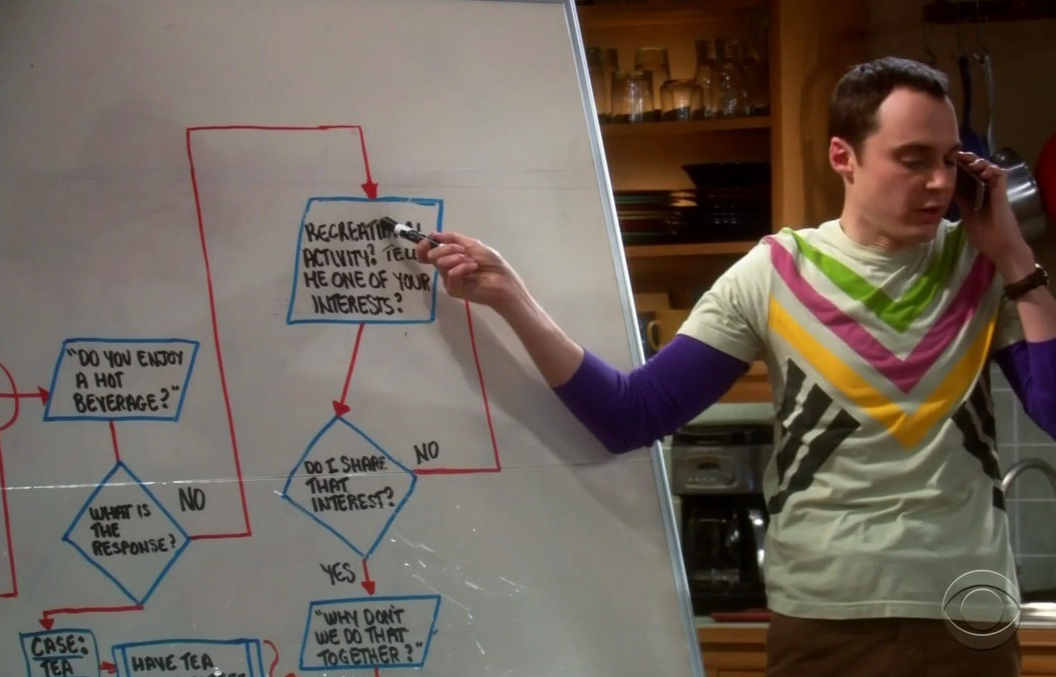
\includegraphics[width=7cm]{fig/Algorithm-sheldon.png}
            
                 \textit{ I believe I've isolateblblblblblblsblbslbslbsl
            sblbslblsblsblblsblbs
            lbslblbslsb d the algorithm for making friends.}
     
            
            \small{
            \hfill Sheldon Cooper, 
            
            \hfill in \textit{The Big Band Theory}, Season 2, Episode 13
            }
}

    \end{columns}

\end{frame}


%%%%%%%%%%%%%%%%%%%%%
\subsection{Introduction}
    \begin{frame}
    \frametitle{Pourquoi faire appel � des algorithmes ?}
    Pour automatiser des t�ches
    
    Exemples :
    \begin{itemize}
    \item M�tier � tisser\\
    \item M�thode de calcul � la main d'une division\\
    \item Recette de cuisine\\
    \item ...\\
    \end{itemize}
    \end{frame}
 
 %%%%%%%%%%%%%%%%%
 
    \begin{frame}
    \frametitle{Qu'est-ce qu'un algorithme ?}
    \begin{block}{D�finition}
    Un algorithme est un ensemble 
    ordonn� d'instructions simples
permettant de r�soudre un probl�me.
    \end{block}
    \end{frame}
    
 %%%%%%%%%%%%%%%%%%
 \subsection{Construction d'un algorithme}
%%%%%%%%%%%%%%%%%%%    
\section{La machine de Turing}
%%%%%%%%%%%%%%%%%%%%
 
  
\begin{frame}[fragile]
\frametitle{Un peu d'histoire...}
\begin{codeblock}{Test}
\begin{codeC}
for (int i = 0 ; i < n ; i ++) {
    //a comment
    printf("%d",i);
    }
\end{codeC}
\end{codeblock}

\begin{termblock}{test 2}
\lstset{escapeinside={��}}
\begin{lstlisting}
�\textbf{>>}�./a.out
�\color{darkgray}{\texttt{  Hello World}}�
\end{lstlisting}
\end{termblock}

 \begin{block}{Bloc standard}
blablabla
\end{block}
\end{frame}


\begin{frame}[fragile]
\frametitle{essai}
\begin{columns}
\column{6cm}
\begin{block}

\begin{figure}
\begin{tikzpicture} [
    auto,
    decision/.style = { diamond, draw=blue, thick, fill=blue!20,
                        text width=5em, text badly centered,
                        inner sep=1pt, rounded corners },
    block/.style    = { rectangle, draw=blue, thick, 
                        fill=blue!20, text width=10em, text centered,
                        rounded corners, minimum height=2em },
    line/.style     = { draw, thick, ->, shorten >=2pt },
  ]
   \matrix [column sep=-10mm, row sep=10mm] {
                    & \node [text centered] (x) {$\mathbf{X}$};            & \\
                    & \node (null1) {};                                    & \\
                    & \node [block] (doa) {\textsf{DoAE}($\mathbf{X}$)};   & \\
  	               \node(null3){}; & \node [decision] (uiddes)
                        {\textsf{UID}($\hat{\mathbf{X}}$)};
                                  & \node[text centered](tra){$\mathbf{i}$}; \\
                  & \node [block] (track) {\textsf{DoAT}($\mathbf{x}$)}; & \\
                    & \node [block] (pesos)
                        {\textsf{BF}(DoA$_{\mathrm{T}}$,DoAs)};            & \\
                    & \node [block] (filtrado)
                        {\textsf{SF}($\mathbf{w}$,$\mathbf{x}$)};          & \\
                    & \node [text centered] (xf) {$\hat{x}(t)$ };          & \\
  };
  % connect all nodes defined above
 \begin{scope} [every path/.style=line]
    \path (x)        --    (doa);
    \path (doa)      --    node [near start] {DoAs} (uiddes);
    \path (tra)      --    (uiddes);
    \path (uiddes)   --++  (-3,0) node [near start] {no} |- (null1);
    \path (uiddes)   --    node [near start] {DoA} (track);
    \path (track)    --    node [near start] {DoA$_{\mathrm{T}}$} (pesos);
    \path (pesos)    --    node [near start] {\textbf{w}} (filtrado);
    \path (filtrado) --    (xf);
  
  \end{scope}
\end{tikzpicture}
\end{figure}
\end{block}
\column{3cm}
\begin{block}{bulbul}
\end{block}
\end{columns}
\end{frame}

\end{document}
